\documentclass[11pt,a4paper]{article}

\usepackage[utf8]{inputenc}
\usepackage{lmodern}
\usepackage[T1]{fontenc}
\usepackage{amsmath,amssymb,amsthm}
\usepackage{mathtools}
\usepackage{stmaryrd}
\usepackage{syntax}
\usepackage{listings}
\usepackage{xcolor}
\usepackage{tikz}
\usetikzlibrary{arrows.meta,positioning,shapes.geometric,fit,calc}
\usepackage{booktabs}
\usepackage{multirow}
\usepackage{caption}
\usepackage{subcaption}
\usepackage[ruled,vlined,linesnumbered]{algorithm2e}
\usepackage{hyperref}
\usepackage[margin=1in]{geometry}
\usepackage{enumitem}
\usepackage{tabularx}

% Theorem environments
\newtheorem{theorem}{Theorem}[section]
\newtheorem{lemma}[theorem]{Lemma}
\newtheorem{proposition}[theorem]{Proposition}
\newtheorem{corollary}[theorem]{Corollary}
\newtheorem{definition}[theorem]{Definition}
\newtheorem{property}[theorem]{Property}

% Listings configuration
\definecolor{kw}{RGB}{0,0,180}
\definecolor{str}{RGB}{0,128,0}
\definecolor{cmt}{RGB}{128,128,128}
\definecolor{bg}{RGB}{248,248,248}

\lstdefinestyle{tsop}{
  backgroundcolor=\color{bg},
  basicstyle=\ttfamily\small,
  keywordstyle=\color{kw}\bfseries,
  stringstyle=\color{str},
  commentstyle=\color{cmt}\itshape,
  breaklines=true,
  frame=single,
  framesep=4pt,
  xleftmargin=8pt,
  xrightmargin=8pt,
  numbers=left,
  numberstyle=\tiny\color{cmt},
  numbersep=6pt,
  tabsize=2,
  showstringspaces=false,
}

\lstdefinestyle{script}{
  backgroundcolor=\color{bg},
  basicstyle=\ttfamily\small,
  keywordstyle=\color{kw}\bfseries,
  breaklines=true,
  frame=single,
  framesep=4pt,
  xleftmargin=8pt,
  xrightmargin=8pt,
  tabsize=2,
  showstringspaces=false,
}

% Semantic macros
\newcommand{\op}[1]{\texttt{OP\_#1}}
\newcommand{\tsop}{\textsc{Tsop}}
\newcommand{\anf}{\textsc{Anf}}
\newcommand{\sir}{\textsc{Sir}} % Stack IR
\newcommand{\bs}{\texttt{ByteString}}
\newcommand{\bigintty}{\texttt{bigint}}
\newcommand{\boolty}{\texttt{boolean}}
\newcommand{\voidty}{\texttt{void}}
\newcommand{\denote}[1]{\llbracket #1 \rrbracket}
\newcommand{\compile}[1]{\mathcal{C}\llbracket #1 \rrbracket}
\newcommand{\typeof}[1]{\Gamma \vdash #1}
\newcommand{\subtype}{\mathrel{<:}}

\title{%
  \textbf{TSOP: A Multi-Frontend Compiler from High-Level\\
  Smart Contract Languages to Bitcoin Script}\\[0.5em]
  \large A Formally Structured Compilation Pipeline with\\
  Cross-Compiler Conformance Guarantees
}

\author{Siggi Oskarsson, BSV Assocation}
\date{March 2026}

\begin{document}

\maketitle

\begin{abstract}
We present \tsop{}, a compiler that translates smart contracts written in
strict subsets of five high-level languages---TypeScript, Solidity, Move, Go,
and Rust---into Bitcoin SV Script. The compilation proceeds through a
six-phase pipeline: parsing, validation, type checking, A-Normal Form (ANF)
lowering, stack lowering, and opcode emission. All five frontends converge
onto a shared Abstract Syntax Tree, which is then lowered through an
ANF-based intermediate representation that serves as the \emph{conformance
boundary} between three independent compiler implementations. We formalize
the type system, describe the stack scheduling algorithm that maps named
temporaries to positional stack operations, and characterize the correctness
properties guaranteed by the pipeline: type safety, termination, determinism,
and UTXO safety. The multi-frontend architecture demonstrates that
language-agnostic smart contract compilation to a stack-based target is
both feasible and practical, enabling developers to write provably
equivalent Bitcoin scripts regardless of source language.
\end{abstract}

\tableofcontents
\newpage

%=============================================================================
\section{Introduction}
\label{sec:intro}
%=============================================================================

Bitcoin Script is a stack-based, non-Turing-complete language embedded in
every Bitcoin transaction. It governs the conditions under which unspent
transaction outputs (UTXOs) may be spent, forming the basis of Bitcoin's
programmable money. Despite its expressive power---particularly in Bitcoin SV,
where the original opcodes have been restored---Bitcoin Script remains
difficult to program directly. Stack manipulation is error-prone, the absence
of named variables forces manual bookkeeping, and the low-level instruction
set lacks the abstractions that developers expect from modern languages.

\tsop{} addresses these challenges through a multi-pass compiler that accepts
smart contracts written in high-level languages and produces Bitcoin Script
locking scripts. The key design decisions are:

\begin{enumerate}[label=(\roman*)]
  \item \textbf{Multi-frontend convergence.} Five distinct source syntaxes
    (TypeScript, Solidity-like, Move-style, Go, Rust) are parsed into a
    single shared AST, enabling polyglot development with identical
    compilation output.
  \item \textbf{ANF as conformance boundary.} The A-Normal Form intermediate
    representation is fully specified and canonically serializable, enabling
    three independent compiler implementations (TypeScript, Go, Rust) to
    produce byte-identical output for the same input.
  \item \textbf{Static guarantees.} The type system, combined with validation
    constraints (bounded loops, no recursion, affine resource types), ensures
    that all compiled programs terminate, maintain type safety, and preserve
    UTXO integrity.
  \item \textbf{Deterministic stack scheduling.} A last-use analysis algorithm
    deterministically maps named ANF temporaries to Bitcoin Script stack
    positions, producing identical bytecode across all three compiler
    implementations.
\end{enumerate}

The remainder of this paper is organized as follows. Section~\ref{sec:language}
defines the source language, its type system, and the contract model.
Section~\ref{sec:frontends} describes each of the five frontend parsers and
their syntax-to-AST mappings. Section~\ref{sec:pipeline} formalizes the
six-phase compilation pipeline. Section~\ref{sec:ir} specifies the three
intermediate representations (AST, ANF IR, Stack IR).
Section~\ref{sec:codegen} details Bitcoin Script code generation, including
the stack scheduling algorithm and opcode emission.
Section~\ref{sec:stateful} describes the compilation of stateful contracts
using the OP\_PUSH\_TX pattern. Section~\ref{sec:correctness} states the
correctness properties of the compilation. Section~\ref{sec:related}
discusses related work, and Section~\ref{sec:conclusion} concludes.

%=============================================================================
\section{Source Language}
\label{sec:language}
%=============================================================================

The \tsop{} source language is a strict, decidable subset of TypeScript
augmented with domain-specific types for Bitcoin Script operations. This
section formalizes the grammar, type system, and contract model.

%-----------------------------------------------------------------------------
\subsection{Grammar}
\label{sec:grammar}
%-----------------------------------------------------------------------------

A \tsop{} program consists of a single contract class extending one of two
base classes. The grammar is given in Figure~\ref{fig:grammar}.

\begin{figure}[h]
\begin{grammar}
<program> ::= <contract>

<contract> ::= `class' <id> `extends' <base-class> `\{' <member>* `\}'

<base-class> ::= `SmartContract' | `StatefulSmartContract'

<member> ::= <property> | <constructor> | <method>

<property> ::= [`readonly'] <id> `:' <type>

<constructor> ::= `constructor' `(' <params> `)' `\{' `super(' <args> `)' `;' <assign>* `\}'

<method> ::= [`public'] <id> `(' <params> `)' [`:' <type>] `\{' <stmt>* `\}'

<stmt> ::= <var-decl> | <assign-stmt> | <if-stmt> | <for-stmt>
       \alt <return-stmt> | <expr-stmt>

<var-decl> ::= (`const' | `let') <id> [`:' <type>] `=' <expr>

<if-stmt> ::= `if' `(' <expr> `)' `\{' <stmt>* `\}' [`else' `\{' <stmt>* `\}']

<for-stmt> ::= `for' `(' <var-decl> `;' <expr> `;' <expr> `)' `\{' <stmt>* `\}'

<expr> ::= <literal> | <id> | <unary-expr> | <binary-expr> | <ternary-expr>
       \alt <call-expr> | <member-expr> | <index-expr> | `(' <expr> `)'

<binary-op> ::= `+' | `-' | `*' | `/' | `\%' | `===' | `!==' | `<' | `>'
           \alt `<=' | `>=' | `\&\&' | `||' | `\&' | `|' | `\^{}' | `<<' | `>>'

<unary-op> ::= `!' | `-' | `\textasciitilde'

<type> ::= `bigint' | `boolean' | `ByteString' | `PubKey' | `Sig'
      \alt `Sha256' | `Ripemd160' | `Addr' | `SigHashPreimage'
      \alt `RabinSig' | `RabinPubKey' | `FixedArray<' <type> `,' <nat> `>'
      \alt `void'
\end{grammar}
\caption{Abstract grammar of the \tsop{} source language.}
\label{fig:grammar}
\end{figure}

The grammar enforces several structural restrictions that are verified
statically during compilation: exactly one contract per file, a constructor
that calls \texttt{super()} as its first statement, and a restricted set of
control flow constructs (no \texttt{while}, \texttt{switch}, \texttt{try/catch},
or unbounded iteration).

%-----------------------------------------------------------------------------
\subsection{Type System}
\label{sec:types}
%-----------------------------------------------------------------------------

The \tsop{} type system is a simple, decidable type system with subtyping
and affine resource tracking. Types are organized into two families with a
strict separation between them.

\begin{definition}[Type Universe]
The set of \tsop{} types $\mathcal{T}$ is partitioned into:
\begin{align}
\mathcal{T}_{\mathrm{int}} &= \{ \bigintty, \texttt{RabinSig}, \texttt{RabinPubKey} \} \\
\mathcal{T}_{\mathrm{bytes}} &= \{ \bs, \texttt{PubKey}, \texttt{Sig}, \texttt{Sha256}, \texttt{Ripemd160}, \texttt{Addr}, \texttt{SigHashPreimage} \} \\
\mathcal{T}_{\mathrm{bool}} &= \{ \boolty \} \\
\mathcal{T}_{\mathrm{array}} &= \{ \texttt{FixedArray}\langle T, n \rangle \mid T \in \mathcal{T}, n \in \mathbb{N} \} \\
\mathcal{T}_{\mathrm{void}} &= \{ \voidty \}
\end{align}
\end{definition}

\begin{definition}[Subtyping Relation]
\label{def:subtyping}
The subtyping relation $\subtype$ is the reflexive-transitive closure of:
\begin{align}
\texttt{RabinSig} &\subtype \bigintty \\
\texttt{RabinPubKey} &\subtype \bigintty \\
\texttt{PubKey} &\subtype \bs \\
\texttt{Sig} &\subtype \bs \\
\texttt{Sha256} &\subtype \bs \\
\texttt{Ripemd160} &\subtype \bs \\
\texttt{Addr} &\subtype \bs \\
\texttt{SigHashPreimage} &\subtype \bs
\end{align}
\end{definition}

This subtyping lattice is shallow (depth at most 1) and decidable in constant
time. Cross-family comparisons are rejected: a value of type \bigintty{}
cannot be compared with a value of type \bs{} using relational operators.

\begin{definition}[Affine Types]
Types $\texttt{SigHashPreimage}$ and $\texttt{Sig}$ are \emph{affine}: values
of these types must be consumed at most once. The type checker tracks usage
and rejects programs that duplicate these values.
\end{definition}

The affine constraint on \texttt{SigHashPreimage} ensures that the sighash
preimage is consumed exactly once in the OP\_PUSH\_TX verification, preventing
transaction malleability. The affine constraint on \texttt{Sig} prevents
signature duplication attacks.

\subsubsection{Typing Rules}

We present selected typing rules using a standard judgment form
$\Gamma \vdash e : \tau$, where $\Gamma$ is a typing environment mapping
identifiers to types.

\begin{gather}
\frac{n \in \mathbb{Z}}{\Gamma \vdash n\texttt{n} : \bigintty}
\quad \textsc{[T-BigInt]}
\qquad
\frac{b \in \{\texttt{true}, \texttt{false}\}}{\Gamma \vdash b : \boolty}
\quad \textsc{[T-Bool]}
\\[1em]
\frac{x : \tau \in \Gamma}{\Gamma \vdash x : \tau}
\quad \textsc{[T-Var]}
\qquad
\frac{\Gamma \vdash e : \tau' \quad \tau' \subtype \tau}{\Gamma \vdash e : \tau}
\quad \textsc{[T-Sub]}
\\[1em]
\frac{
  \Gamma \vdash e_1 : \bigintty \quad
  \Gamma \vdash e_2 : \bigintty \quad
  \oplus \in \{+, -, *, /, \%, \mathbin{\&}, |, \hat{}, \ll, \gg\}
}{
  \Gamma \vdash e_1 \oplus e_2 : \bigintty
}
\quad \textsc{[T-Arith]}
\\[1em]
\frac{
  \Gamma \vdash e_1 : \bigintty \quad
  \Gamma \vdash e_2 : \bigintty \quad
  \oplus \in \{<, >, \leq, \geq\}
}{
  \Gamma \vdash e_1 \oplus e_2 : \boolty
}
\quad \textsc{[T-Rel]}
\\[1em]
\frac{
  \Gamma \vdash e_1 : \tau_1 \quad
  \Gamma \vdash e_2 : \tau_2 \quad
  \tau_1 \sim \tau_2 \quad
  \oplus \in \{===, !==\}
}{
  \Gamma \vdash e_1 \oplus e_2 : \boolty
}
\quad \textsc{[T-Eq]}
\end{gather}

where $\tau_1 \sim \tau_2$ (type compatibility) holds when $\tau_1 \subtype \tau_2$ or $\tau_2 \subtype \tau_1$, and both types belong to the same family ($\mathcal{T}_{\mathrm{int}}$ or $\mathcal{T}_{\mathrm{bytes}}$ or $\mathcal{T}_{\mathrm{bool}}$).

\subsubsection{Built-in Function Typing}

\tsop{} provides a closed set of built-in functions. No user-defined
free-standing functions are permitted; the type checker rejects calls to any
function not in this set or not a method on the current contract.

\begin{table}[h]
\centering
\small
\begin{tabularx}{\textwidth}{@{}llX@{}}
\toprule
\textbf{Category} & \textbf{Function} & \textbf{Signature} \\
\midrule
\multirow{4}{*}{Hashing}
  & \texttt{sha256} & $\bs \to \texttt{Sha256}$ \\
  & \texttt{hash160} & $\bs \to \texttt{Ripemd160}$ \\
  & \texttt{hash256} & $\bs \to \texttt{Sha256}$ \\
  & \texttt{ripemd160} & $\bs \to \texttt{Ripemd160}$ \\
\midrule
\multirow{3}{*}{Signatures}
  & \texttt{checkSig} & $\texttt{Sig} \times \texttt{PubKey} \to \boolty$ \\
  & \texttt{checkMultiSig} & $\texttt{Sig}[] \times \texttt{PubKey}[] \to \boolty$ \\
  & \texttt{verifyRabinSig} & $\bs \times \texttt{RabinSig} \times \bs \times \texttt{RabinPubKey} \to \boolty$ \\
\midrule
\multirow{4}{*}{Mathematics}
  & \texttt{abs}, \texttt{min}, \texttt{max} & $\bigintty^{(1\text{--}2)} \to \bigintty$ \\
  & \texttt{within} & $\bigintty \times \bigintty \times \bigintty \to \boolty$ \\
  & \texttt{pow}, \texttt{sqrt}, \texttt{gcd} & $\bigintty^{(1\text{--}2)} \to \bigintty$ \\
  & \texttt{safediv}, \texttt{safemod}, \texttt{mulDiv} & $\bigintty^{(2\text{--}3)} \to \bigintty$ \\
\midrule
\multirow{3}{*}{Byte Ops}
  & \texttt{len} & $\bs \to \bigintty$ \\
  & \texttt{cat} & $\bs \times \bs \to \bs$ \\
  & \texttt{num2bin}, \texttt{bin2num} & $\bigintty \times \bigintty \to \bs$ / $\bs \to \bigintty$ \\
\midrule
Post-Quantum
  & \texttt{verifyWOTS} & $\bs \times \bs \times \bs \to \boolty$ \\
\midrule
Control
  & \texttt{assert} & $\boolty \to \voidty$ \\
\bottomrule
\end{tabularx}
\caption{Selected built-in function signatures (abbreviated).}
\label{tab:builtins}
\end{table}

%-----------------------------------------------------------------------------
\subsection{Contract Model}
\label{sec:contract-model}
%-----------------------------------------------------------------------------

\tsop{} defines two contract base classes that correspond to distinct
Bitcoin Script patterns.

\begin{definition}[Stateless Contract]
A \emph{stateless contract} (\texttt{SmartContract}) has the following
properties:
\begin{enumerate}[label=(\alph*)]
  \item All properties are \texttt{readonly} and embedded as constants in
    the locking script at deployment time.
  \item Public methods are spending conditions: each is a predicate that must
    evaluate to \texttt{true} for the UTXO to be spent.
  \item No state transitions occur; the script is evaluated once and discarded.
\end{enumerate}
\end{definition}

\begin{definition}[Stateful Contract]
A \emph{stateful contract} (\texttt{StatefulSmartContract}) extends the
stateless model with:
\begin{enumerate}[label=(\alph*)]
  \item At least one mutable (non-\texttt{readonly}) property.
  \item Automatic injection of \texttt{checkPreimage} verification at the
    entry of every public method, implementing the OP\_PUSH\_TX pattern.
  \item Automatic state continuation: at method exit, the compiler emits
    code that serializes the updated state, constructs the expected
    transaction output, and verifies it matches the spending transaction's
    output hash.
\end{enumerate}
\end{definition}

The \texttt{parentClass} field on the AST's \texttt{ContractNode}
discriminates between these two models, determining which compilation
strategy is applied in later passes.

%=============================================================================
\section{Multi-Frontend Architecture}
\label{sec:frontends}
%=============================================================================

A key design contribution of \tsop{} is the separation of surface syntax
from the compilation pipeline. Five distinct frontend parsers translate
source code into a shared AST representation, after which the remaining
five passes are syntax-agnostic. This section describes each frontend's
syntax and its mapping to the canonical AST.

\begin{figure}[h]
\centering
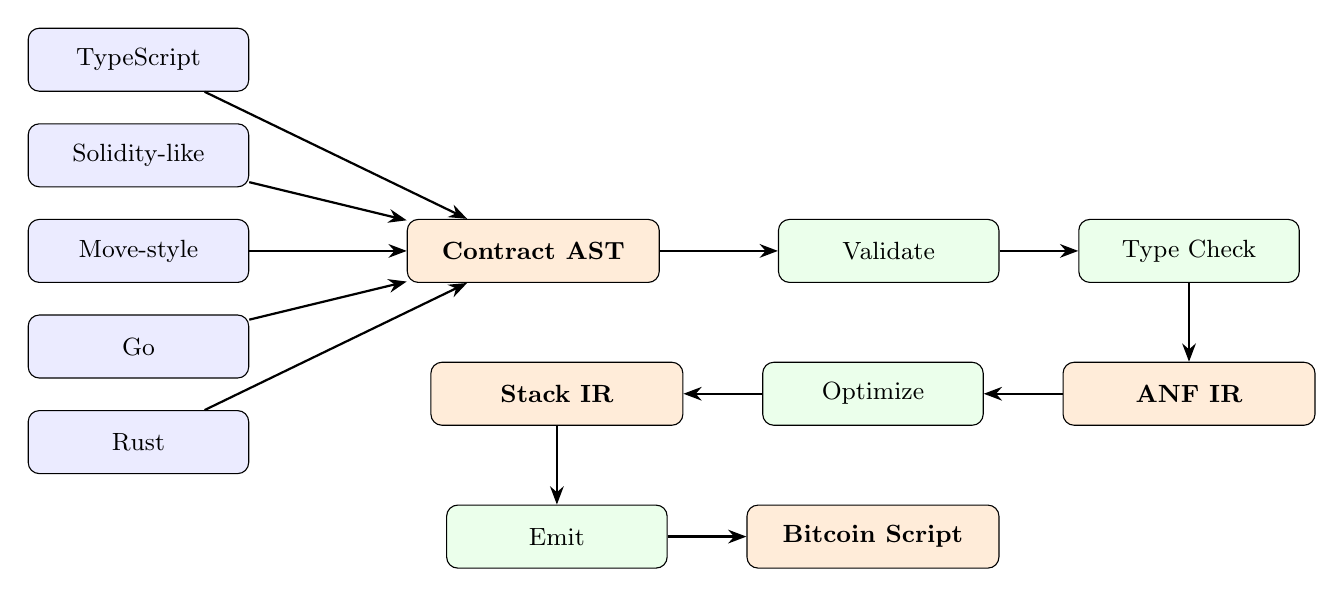
\begin{tikzpicture}[
  node distance=0.8cm and 1.5cm,
  frontend/.style={draw, rounded corners, fill=blue!8, minimum width=2.8cm, minimum height=0.8cm, font=\small},
  ir/.style={draw, rounded corners, fill=orange!15, minimum width=3.2cm, minimum height=0.8cm, font=\small\bfseries},
  pass/.style={draw, rounded corners, fill=green!8, minimum width=2.8cm, minimum height=0.8cm, font=\small},
  arrow/.style={-Stealth, thick},
]
  % Frontends
  \node[frontend] (ts) {TypeScript};
  \node[frontend, below=0.4cm of ts] (sol) {Solidity-like};
  \node[frontend, below=0.4cm of sol] (move) {Move-style};
  \node[frontend, below=0.4cm of move] (go) {Go};
  \node[frontend, below=0.4cm of go] (rs) {Rust};

  % AST
  \node[ir, right=2cm of move] (ast) {Contract AST};

  % Pipeline
  \node[pass, right=1.5cm of ast] (val) {Validate};
  \node[pass, right=1cm of val] (tc) {Type Check};
  \node[ir, below=1cm of tc] (anf) {ANF IR};
  \node[pass, left=1cm of anf] (opt) {Optimize};
  \node[ir, left=1cm of opt] (stack) {Stack IR};
  \node[pass, below=1cm of stack] (emit) {Emit};
  \node[ir, right=1cm of emit] (btc) {Bitcoin Script};

  % Frontend arrows
  \foreach \f in {ts, sol, move, go, rs}
    \draw[arrow] (\f) -- (ast);

  % Pipeline arrows
  \draw[arrow] (ast) -- (val);
  \draw[arrow] (val) -- (tc);
  \draw[arrow] (tc) -- (anf);
  \draw[arrow] (anf) -- (opt);
  \draw[arrow] (opt) -- (stack);
  \draw[arrow] (stack) -- (emit);
  \draw[arrow] (emit) -- (btc);

\end{tikzpicture}
\caption{Multi-frontend compilation pipeline. All five frontends converge
  onto the shared Contract AST; subsequent passes are syntax-agnostic.}
\label{fig:pipeline}
\end{figure}

%-----------------------------------------------------------------------------
\subsection{TypeScript Frontend}
\label{sec:frontend-ts}
%-----------------------------------------------------------------------------

The canonical \tsop{} syntax uses a strict subset of TypeScript. Contracts
are declared as classes extending one of the two base classes:

\begin{lstlisting}[style=tsop,language=Java,
  morekeywords={class,extends,constructor,super,readonly,public,private,const,let,if,else,for,return,assert,bigint,boolean}]
class P2PKH extends SmartContract {
  readonly pubKeyHash: Ripemd160;

  constructor(pubKeyHash: Ripemd160) {
    super(pubKeyHash);
    this.pubKeyHash = pubKeyHash;
  }

  public unlock(sig: Sig, pubKey: PubKey) {
    assert(hash160(pubKey) === this.pubKeyHash);
    assert(checkSig(sig, pubKey));
  }
}
\end{lstlisting}

The TypeScript frontend maps directly to the AST with minimal transformation:
\texttt{readonly} maps to the property's \texttt{readonly} flag,
\texttt{public}/\texttt{private} keywords control method visibility, and
TypeScript type annotations are preserved verbatim as \tsop{} types.
Numeric literals (both \texttt{42n} and \texttt{42}) are uniformly
interpreted as \bigintty{}.

%-----------------------------------------------------------------------------
\subsection{Solidity-like Frontend}
\label{sec:frontend-sol}
%-----------------------------------------------------------------------------

The Solidity-like frontend accepts a syntax inspired by Ethereum's Solidity,
with adaptations for the \tsop{} type system:

\begin{lstlisting}[style=tsop,language=Java,
  morekeywords={pragma,contract,is,immutable,function,public,private,returns,require,int,bool,bytes}]
pragma tsop ^0.1.0;

contract P2PKH is SmartContract {
  Ripemd160 immutable pubKeyHash;

  function unlock(Sig sig, PubKey pubKey) public {
    require(hash160(pubKey) == pubKeyHash);
    require(checkSig(sig, pubKey));
  }
}
\end{lstlisting}

Table~\ref{tab:sol-mapping} summarizes the key syntactic mappings.

\begin{table}[h]
\centering
\small
\begin{tabular}{@{}lll@{}}
\toprule
\textbf{Solidity Syntax} & \textbf{AST Mapping} & \textbf{Notes} \\
\midrule
\texttt{immutable} & \texttt{readonly: true} & Before field name \\
\texttt{require(e)} & \texttt{assert(e)} & Direct substitution \\
\texttt{==}, \texttt{!=} & \texttt{===}, \texttt{!==} & Strict equality \\
\texttt{int}, \texttt{uint}, \texttt{int256} & \bigintty & All integer types unified \\
\texttt{bool} & \boolty & Direct mapping \\
\texttt{bytes} & \bs & Direct mapping \\
\texttt{address} & \texttt{Addr} & 20-byte type \\
\texttt{Type[N]} & \texttt{FixedArray<Type,N>} & Array syntax \\
\bottomrule
\end{tabular}
\caption{Solidity-like frontend: syntax-to-AST mappings.}
\label{tab:sol-mapping}
\end{table}

The parser is implemented as a hand-written recursive descent parser with a
custom lexer. A precedence-climbing algorithm handles operator precedence.
The constructor is auto-generated from the struct fields if not explicitly
provided, with \texttt{super()} injected as the first statement.

%-----------------------------------------------------------------------------
\subsection{Move-style Frontend}
\label{sec:frontend-move}
%-----------------------------------------------------------------------------

The Move-style frontend uses a syntax inspired by the Move language, with
module declarations and resource structs:

\begin{lstlisting}[style=tsop,language=Java,
  morekeywords={module,use,resource,struct,public,fun,let,mut,assert}]
module P2PKH {
  use tsop::SmartContract;

  resource struct P2PKH {
    pub_key_hash: Ripemd160 readonly,
  }

  public fun unlock(sig: Sig, pub_key: PubKey) {
    assert!(hash160(pub_key) == self.pub_key_hash);
    assert!(check_sig(sig, pub_key));
  }
}
\end{lstlisting}

A distinguishing feature of the Move frontend is automatic identifier
conversion from \texttt{snake\_case} to \texttt{camelCase}:
\texttt{pub\_key\_hash} becomes \texttt{pubKeyHash},
\texttt{check\_sig} becomes \texttt{checkSig}, and so forth. The
\texttt{assert!} macro is mapped to \texttt{assert()}, and
\texttt{assert\_eq!(a, b)} is desugared to \texttt{assert(a === b)}.

Type mappings include \texttt{Int} $\to$ \bigintty{},
\texttt{Bool} $\to$ \boolty{}, and \texttt{vector} $\to$ \bs{}.
Reference types (\texttt{\&T}, \texttt{\&mut T}) are stripped during parsing.
The presence of mutable fields (\texttt{\&mut}) or the use of
\texttt{StatefulSmartContract} determines the contract model.

%-----------------------------------------------------------------------------
\subsection{Go Frontend}
\label{sec:frontend-go}
%-----------------------------------------------------------------------------

The Go frontend parses Go source code using the standard Go parser from
the \texttt{go/parser} package, then maps the Go AST to the \tsop{} AST:

\begin{lstlisting}[style=tsop,language=Go,
  morekeywords={type,struct,func}]
type P2PKH struct {
  tsop.SmartContract
  PubKeyHash tsop.Ripemd160 `tsop:"readonly"`
}

func (c *P2PKH) Unlock(sig tsop.Sig, pubKey tsop.PubKey) {
  tsop.Assert(tsop.Hash160(pubKey) == c.PubKeyHash)
  tsop.Assert(tsop.CheckSig(sig, pubKey))
}
\end{lstlisting}

Key mapping rules include:

\begin{itemize}[nosep]
  \item \textbf{Embedding}: \texttt{tsop.SmartContract} as an anonymous
    field determines the base class.
  \item \textbf{Struct tags}: \texttt{`tsop:"readonly"`} marks immutable
    properties.
  \item \textbf{Visibility}: Exported (capitalized) methods are public;
    unexported methods are private.
  \item \textbf{Name conversion}: \texttt{PascalCase} $\to$
    \texttt{camelCase} for method and field names.
  \item \textbf{Selector resolution}: \texttt{tsop.X} selectors are mapped
    to built-in function calls; non-\texttt{tsop} selectors are rejected.
  \item \textbf{Type conversions}: \texttt{tsop.Int(0)} unwraps to the
    inner value; \texttt{tsop.Bool(expr)} similarly unwraps.
\end{itemize}

%-----------------------------------------------------------------------------
\subsection{Rust Frontend}
\label{sec:frontend-rs}
%-----------------------------------------------------------------------------

The Rust frontend uses attribute macros to annotate standard Rust structs and
impl blocks:

\begin{lstlisting}[style=tsop,language=Rust,
  morekeywords={pub,struct,impl,fn,let,mut,self}]
#[tsop::contract]
pub struct P2PKH {
  #[readonly]
  pub pub_key_hash: Ripemd160,
}

#[tsop::methods(P2PKH)]
impl P2PKH {
  #[public]
  pub fn unlock(&self, sig: &Sig, pub_key: &PubKey) {
    assert!(hash160(pub_key) == self.pub_key_hash);
    assert!(check_sig(sig, pub_key));
  }
}
\end{lstlisting}

The Rust frontend shares the \texttt{snake\_case} $\to$ \texttt{camelCase}
conversion with the Move frontend. Reference types (\texttt{\&T}) are
stripped, and \texttt{.clone()} calls are treated as no-ops (necessary for
Rust's borrow checker but irrelevant to Bitcoin Script semantics).
The \texttt{\#[readonly]} attribute on fields is stripped by the proc-macro
(Rust does not allow \texttt{proc\_macro\_attribute} on struct fields
natively), and \texttt{\#[public]} controls method visibility.
Range-based for loops (\texttt{for i in 0..n}) are translated to
bounded C-style loops in the AST.

%-----------------------------------------------------------------------------
\subsection{Frontend Convergence}
\label{sec:convergence}
%-----------------------------------------------------------------------------

\begin{property}[Frontend Equivalence]
\label{prop:frontend-equiv}
For any contract $C$ expressible in all five frontend syntaxes, let
$\text{parse}_f(C_f)$ denote the AST produced by frontend $f$. Then:
\[
  \forall f_1, f_2 \in \{\text{TS}, \text{Sol}, \text{Move}, \text{Go}, \text{Rust}\}:
  \quad \text{normalize}(\text{parse}_{f_1}(C_{f_1})) = \text{normalize}(\text{parse}_{f_2}(C_{f_2}))
\]
where $\text{normalize}$ canonicalizes identifier names (via the
\texttt{camelCase} convention), strips source locations, and orders
properties by declaration.
\end{property}

This property is verified by the cross-compiler conformance test suite,
which compiles the same contracts in all available formats and compares
the byte-identical output at the ANF IR and Bitcoin Script levels.

%=============================================================================
\section{Compilation Pipeline}
\label{sec:pipeline}
%=============================================================================

The \tsop{} compilation pipeline consists of six pure-function passes.
Each pass transforms a well-defined input into a well-defined output,
with no shared mutable state between passes.

%-----------------------------------------------------------------------------
\subsection{Pass 1: Parse}
\label{sec:pass-parse}
%-----------------------------------------------------------------------------

The parser accepts a source string and an optional filename. The filename's
extension determines which frontend parser is invoked:

\begin{center}
\begin{tabular}{@{}ll@{}}
\toprule
\textbf{Extension} & \textbf{Parser} \\
\midrule
\texttt{.tsop.ts} (or default) & TypeScript (via ts-morph) \\
\texttt{.tsop.sol} & Solidity-like (recursive descent) \\
\texttt{.tsop.move} & Move-style (recursive descent) \\
\texttt{.tsop.go} & Go (\texttt{go/parser} + AST mapping) \\
\texttt{.tsop.rs} & Rust (tokenizer + recursive descent) \\
\bottomrule
\end{tabular}
\end{center}

All parsers produce a \texttt{ContractNode} AST (defined in
Section~\ref{sec:ir-ast}) or a list of diagnostic errors.
The parser extracts exactly one contract per source file.

%-----------------------------------------------------------------------------
\subsection{Pass 2: Validate}
\label{sec:pass-validate}
%-----------------------------------------------------------------------------

The validation pass enforces language subset constraints without modifying
the AST. The following invariants are checked:

\begin{enumerate}[label=\textbf{V\arabic*}., ref=V\arabic*]
  \item \label{v:types} All property types are valid \tsop{} types (no
    \texttt{void}, \texttt{any}, \texttt{number}, \texttt{string}).
  \item \label{v:super} The constructor calls \texttt{super()} as its first
    statement.
  \item \label{v:assign} Each property is assigned exactly once in the
    constructor.
  \item \label{v:readonly} All properties in \texttt{SmartContract} are
    \texttt{readonly}; \texttt{StatefulSmartContract} has at least one
    mutable property.
  \item \label{v:recursion} No direct or mutual recursion among methods.
  \item \label{v:loops} All \texttt{for} loop bounds are compile-time
    constants.
  \item \label{v:subset} No disallowed constructs: \texttt{while},
    \texttt{do-while}, \texttt{switch}, \texttt{try/catch},
    \texttt{async/await}, decorators, closures, \texttt{typeof},
    \texttt{instanceof}, or arbitrary imports.
\end{enumerate}

\begin{proposition}[Termination from Validation]
\label{prop:termination}
If a program passes validation, its execution terminates. This follows from
\ref{v:loops} (all loops are bounded) and \ref{v:recursion} (no recursion),
which together ensure that the call graph is acyclic and all iteration is
finite.
\end{proposition}

%-----------------------------------------------------------------------------
\subsection{Pass 3: Type Check}
\label{sec:pass-typecheck}
%-----------------------------------------------------------------------------

The type checker verifies type consistency according to the rules in
Section~\ref{sec:types}. It proceeds in four phases:

\begin{enumerate}[nosep]
  \item \textbf{Declaration collection}: Build a typing environment $\Gamma$
    from contract properties.
  \item \textbf{Constructor verification}: Check \texttt{super()} arguments
    and property assignments.
  \item \textbf{Method body checking}: For each method, extend $\Gamma$ with
    parameters and local variables; type-check each statement and expression.
  \item \textbf{Whole-program checks}: Verify affine type consumption,
    code size bounds, and unknown function rejection.
\end{enumerate}

The type checker maintains a map of approximately 50 built-in function
signatures. Any call to a function not in this map, not a contract method,
and not a local variable is rejected. This \emph{closed-world assumption}
ensures that the compiled script contains no references to functions that
cannot be realized in Bitcoin Script.

%-----------------------------------------------------------------------------
\subsection{Pass 4: ANF Lowering}
\label{sec:pass-anf}
%-----------------------------------------------------------------------------

The ANF lowering pass transforms the typed AST into A-Normal Form, a
representation in which every sub-expression is bound to a named temporary:

\begin{definition}[A-Normal Form]
An ANF program consists of a sequence of \emph{bindings} $b_0, b_1, \ldots, b_n$
where each binding has the form:
\[
  \texttt{let } t_i = V_i
\]
and $V_i$ is a \emph{simple value}---an operation whose arguments are
exclusively variable references (to parameters, properties, or earlier
temporaries $t_j$ where $j < i$).
\end{definition}

The transformation eliminates all nested expressions. For example:
\begin{align*}
  \texttt{assert(hash160(pubKey) === this.pubKeyHash)}
\end{align*}
becomes:
\begin{align*}
  \texttt{let } t_0 &= \texttt{load\_param(pubKey)} \\
  \texttt{let } t_1 &= \texttt{call(hash160, [}t_0\texttt{])} \\
  \texttt{let } t_2 &= \texttt{load\_prop(pubKeyHash)} \\
  \texttt{let } t_3 &= \texttt{bin\_op(===, }t_1, t_2\texttt{)} \\
  \texttt{let } t_4 &= \texttt{assert(}t_3\texttt{)}
\end{align*}

Temporaries are numbered sequentially ($t_0, t_1, t_2, \ldots$) within each
method. This canonical naming scheme is critical for cross-compiler
conformance: all three compiler implementations must produce identical
temporary indices for the same input.

\subsubsection{Short-Circuit Lowering}

Logical operators are desugared into conditional expressions:
\begin{align}
  a \mathbin{\&\&} b &\leadsto \texttt{if}(a)\; \{b\}\; \texttt{else}\; \{\texttt{false}\} \\
  a \mathbin{||} b &\leadsto \texttt{if}(a)\; \{\texttt{true}\}\; \texttt{else}\; \{b\}
\end{align}

\subsubsection{Stateful Contract Injection}

For contracts extending \texttt{StatefulSmartContract}, the ANF lowering
pass automatically injects additional bindings at the entry and exit of
every public method:

\textbf{Entry injection:}
\begin{align*}
  \texttt{let } t_0 &= \texttt{load\_param(txPreimage)} \\
  \texttt{let } t_1 &= \texttt{check\_preimage(}t_0\texttt{)} \\
  \texttt{let } t_2 &= \texttt{assert(}t_1\texttt{)}
\end{align*}

\textbf{Exit injection} (single-output state continuation):
\begin{align*}
  \texttt{let } t_k &= \texttt{get\_state\_script()} \\
  \texttt{let } t_{k+1} &= \texttt{call(hash256, [}t_k\texttt{])} \\
  \texttt{let } t_{k+2} &= \texttt{load\_param(txPreimage)} \\
  \texttt{let } t_{k+3} &= \texttt{call(extractOutputHash, [}t_{k+2}\texttt{])} \\
  \texttt{let } t_{k+4} &= \texttt{bin\_op(===, }t_{k+1}, t_{k+3}\texttt{)}  \\
  \texttt{let } t_{k+5} &= \texttt{assert(}t_{k+4}\texttt{)}
\end{align*}

%-----------------------------------------------------------------------------
\subsection{Pass 4.5: Constant Folding (Optimizer)}
\label{sec:pass-optimize}
%-----------------------------------------------------------------------------

Between ANF lowering and stack lowering, an optional constant folding
optimizer evaluates compile-time-known expressions:

\begin{definition}[Constant Folding]
A binding $\texttt{let } t_i = V_i$ is \emph{foldable} if $V_i$ is a
binary operation, unary operation, or pure built-in call whose arguments
are all constants (i.e., \texttt{load\_const} bindings). The optimizer
replaces $V_i$ with a \texttt{load\_const} of the computed result.
\end{definition}

The optimizer handles all arithmetic, comparison, and bitwise operations on
constants, as well as pure mathematical built-ins (\texttt{abs}, \texttt{min},
\texttt{max}, \texttt{pow}, \texttt{sqrt}, \texttt{gcd}, etc.). Constants
are propagated through the binding sequence, enabling cascading optimizations.

The optimizer preserves the binding indices---it replaces values in-place
rather than removing bindings---ensuring that subsequent bindings' references
remain valid.

%-----------------------------------------------------------------------------
\subsection{Pass 5: Stack Lowering}
\label{sec:pass-stack}
%-----------------------------------------------------------------------------

The stack lowering pass is the most complex transformation in the pipeline.
It converts the named-variable ANF representation into a positional stack
representation suitable for Bitcoin Script emission.

\subsubsection{Stack Model}

Bitcoin Script provides a main stack and an alt stack. The compiler models
the main stack as a sequence of named values indexed from the top
(position 0) downward:

\begin{definition}[Stack Map]
A \emph{stack map} $\sigma : \mathbb{N} \to \text{Name}$ maps each stack
position (0 = top) to the name of the value stored there. The compiler
maintains $\sigma$ as a virtual tracking structure during lowering.
\end{definition}

\subsubsection{Last-Use Analysis}

Before generating stack operations, the compiler performs a last-use analysis:

\begin{definition}[Last Use]
For each variable $v$ defined at binding index $d$ and referenced at binding
indices $u_1, u_2, \ldots, u_k$ (where $u_1 < u_2 < \cdots < u_k$), the
\emph{last use} of $v$ is $u_k$. At binding $u_k$, the value of $v$ may be
consumed (removed from the stack); at all earlier uses, it must be copied.
\end{definition}

This analysis determines whether a value is accessed via \op{ROLL}
(consuming, for last use) or \op{PICK} (copying, for non-last use).
The choice between these operations is the primary source of optimization
in stack lowering.

\subsubsection{Value Retrieval}

To bring a value to the top of the stack, the compiler uses Algorithm~\ref{alg:bring}.

\begin{algorithm}[h]
\SetAlgoLined
\KwIn{Variable name $v$, boolean \textit{consume}, stack map $\sigma$}
\KwOut{Sequence of stack operations}
$d \gets \sigma^{-1}(v)$ \tcp*{Find position of $v$ in $\sigma$}
\uIf{$d = 0$}{
  \uIf{\textit{consume}}{
    \Return $\varepsilon$ \tcp*{Already on top; will be consumed by next op}
  }\Else{
    \Return \op{DUP} \tcp*{Copy top item}
  }
}
\uElseIf{$d = 1$ \textbf{and} \textit{consume}}{
  \Return \op{SWAP} \tcp*{1-byte swap is cheaper than 2-byte ROLL}
}
\uElseIf{$d = 1$ \textbf{and not} \textit{consume}}{
  \Return \op{OVER} \tcp*{Copy second item}
}
\uElseIf{$d = 2$ \textbf{and} \textit{consume}}{
  \Return \op{ROT} \tcp*{Rotate top 3 (equivalent to ROLL 2)}
}
\Else{
  \uIf{\textit{consume}}{
    \Return $\texttt{push}(d);\; \op{ROLL}$
  }\Else{
    \Return $\texttt{push}(d);\; \op{PICK}$
  }
}
Update $\sigma$ accordingly\;
\caption{BringToTop: Retrieve a value from the stack}
\label{alg:bring}
\end{algorithm}

\subsubsection{Lowering Bindings}

Each ANF binding is lowered by:
\begin{enumerate}[nosep]
  \item Bringing required operands to the top of the stack using
    Algorithm~\ref{alg:bring}, consulting the last-use analysis to
    determine whether to consume or copy.
  \item Emitting the appropriate opcode(s) for the operation.
  \item Recording the result's name in the stack map.
\end{enumerate}

%-----------------------------------------------------------------------------
\subsection{Pass 6: Emit}
\label{sec:pass-emit}
%-----------------------------------------------------------------------------

The emission pass serializes Stack IR operations into Bitcoin Script bytecode.
Two peephole optimizations are applied during emission:

\begin{enumerate}[nosep]
  \item \textbf{Verify fusion}: \op{EQUAL}\,\op{VERIFY} $\to$
    \op{EQUALVERIFY}, \op{NUMEQUAL}\,\op{VERIFY} $\to$
    \op{NUMEQUALVERIFY}, \op{CHECKSIG}\,\op{VERIFY} $\to$
    \op{CHECKSIGVERIFY}. Each fusion saves one byte.
  \item \textbf{Swap elimination}: \op{SWAP}\,\op{SWAP} $\to \varepsilon$.
    Consecutive swaps cancel out.
\end{enumerate}

Data encoding follows the Bitcoin Script number format:

\begin{definition}[Script Number Encoding]
A \bigintty{} value $n$ is encoded as a little-endian, sign-magnitude
byte sequence with minimal encoding:
\begin{itemize}[nosep]
  \item $n = 0$: \op{0} (opcode \texttt{0x00}, pushes empty byte array)
  \item $1 \leq n \leq 16$: \op{$n$} (opcodes \texttt{0x51}--\texttt{0x60})
  \item $n = -1$: \op{1NEGATE} (opcode \texttt{0x4f})
  \item Otherwise: little-endian bytes, with sign bit in MSB. If the MSB's
    high bit is set, an additional \texttt{0x00} (positive) or \texttt{0x80}
    (negative) byte is appended.
\end{itemize}
\end{definition}

Byte string data is pushed using direct push ($\leq 75$ bytes),
\op{PUSHDATA1} (76--255 bytes), \op{PUSHDATA2} (256--65535 bytes),
or \op{PUSHDATA4} ($> 65535$ bytes).

%=============================================================================
\section{Intermediate Representations}
\label{sec:ir}
%=============================================================================

The compilation pipeline uses three intermediate representations, each at a
different level of abstraction.

%-----------------------------------------------------------------------------
\subsection{Contract AST}
\label{sec:ir-ast}
%-----------------------------------------------------------------------------

The Contract AST is a tree-structured representation with the following
principal node types:

\[
\begin{array}{rcl}
\texttt{ContractNode} &=& \langle \textit{name}, \textit{parentClass}, \textit{properties}^*, \textit{constructor}, \textit{methods}^* \rangle \\
\texttt{PropertyNode} &=& \langle \textit{name}, \textit{type}, \textit{readonly} \rangle \\
\texttt{MethodNode} &=& \langle \textit{name}, \textit{params}^*, \textit{body}^*, \textit{visibility} \rangle \\
\texttt{Statement} &=& \texttt{VarDecl} \mid \texttt{Assign} \mid \texttt{If} \mid \texttt{For} \mid \texttt{Return} \mid \texttt{ExprStmt} \\
\texttt{Expression} &=& \texttt{BinExpr} \mid \texttt{UnaryExpr} \mid \texttt{CallExpr} \mid \texttt{Ident} \mid \texttt{Literal} \mid \cdots
\end{array}
\]

%-----------------------------------------------------------------------------
\subsection{ANF IR}
\label{sec:ir-anf}
%-----------------------------------------------------------------------------

The ANF IR is a flat, canonically serializable representation. Its structure
is:

\[
\begin{array}{rcl}
\texttt{ANFProgram} &=& \langle \textit{version}, \textit{contractName}, \textit{properties}^*, \textit{methods}^* \rangle \\
\texttt{ANFMethod} &=& \langle \textit{name}, \textit{params}^*, \textit{body}^*, \textit{isPublic} \rangle \\
\texttt{ANFBinding} &=& \langle t_i, V_i \rangle
\end{array}
\]

The value kinds $V$ are:

\begin{center}
\small
\begin{tabular}{@{}ll@{}}
\toprule
\textbf{Kind} & \textbf{Description} \\
\midrule
\texttt{load\_param}$(x)$ & Load method parameter $x$ \\
\texttt{load\_prop}$(x)$ & Load contract property $x$ \\
\texttt{load\_const}$(c)$ & Push compile-time constant $c$ \\
\texttt{bin\_op}$(\oplus, l, r)$ & Binary operation on temporaries $l, r$ \\
\texttt{unary\_op}$(\ominus, x)$ & Unary operation on temporary $x$ \\
\texttt{call}$(f, \vec{a})$ & Built-in function call \\
\texttt{method\_call}$(m, \vec{a})$ & Private method call (inlined) \\
\texttt{if}$(c, \vec{t}, \vec{e})$ & Conditional with then/else binding sequences \\
\texttt{loop}$(n, \vec{b}, i)$ & Unrolled loop of $n$ iterations \\
\texttt{assert}$(x)$ & Runtime assertion \\
\texttt{update\_prop}$(p, v)$ & Mutable property update \\
\texttt{get\_state\_script}$ ()$ & Serialize state to bytes \\
\texttt{check\_preimage}$(x)$ & Verify sighash preimage \\
\texttt{add\_output}$(s, \vec{v})$ & Emit transaction output \\
\bottomrule
\end{tabular}
\end{center}

The ANF IR is serialized using RFC 8785 (JSON Canonicalization Scheme)
with lexicographically sorted keys, no whitespace, and minimal number
representations. This canonical form serves as the \emph{conformance
boundary}: all three compiler implementations must produce byte-identical
ANF IR JSON for the same input.

%-----------------------------------------------------------------------------
\subsection{Stack IR}
\label{sec:ir-stack}
%-----------------------------------------------------------------------------

The Stack IR is a flat sequence of stack machine operations:

\[
\begin{array}{rcl}
\texttt{StackOp} &=& \texttt{push}(v) \mid \texttt{dup} \mid \texttt{swap} \mid \texttt{roll}(d) \mid \texttt{pick}(d) \\
  &\mid& \texttt{drop} \mid \texttt{nip} \mid \texttt{over} \mid \texttt{rot} \mid \texttt{tuck} \\
  &\mid& \texttt{opcode}(c) \mid \texttt{if}(\vec{t}, \vec{e})
\end{array}
\]

where $v$ is a push value (integer, boolean, or byte sequence), $d$ is a
stack depth, $c$ is a Bitcoin Script opcode name, and $\vec{t}, \vec{e}$
are sequences of stack operations for the then/else branches.

%=============================================================================
\section{Bitcoin Script Code Generation}
\label{sec:codegen}
%=============================================================================

This section details how specific language constructs are compiled to
Bitcoin Script opcode sequences.

%-----------------------------------------------------------------------------
\subsection{Operator Compilation}
\label{sec:codegen-ops}
%-----------------------------------------------------------------------------

Binary operators map directly to Bitcoin Script opcodes:

\begin{center}
\small
\begin{tabular}{@{}ll@{\qquad}ll@{}}
\toprule
\textbf{Operator} & \textbf{Opcode} & \textbf{Operator} & \textbf{Opcode} \\
\midrule
\texttt{+} & \op{ADD} & \texttt{===} (int) & \op{NUMEQUAL} \\
\texttt{-} & \op{SUB} & \texttt{===} (bytes) & \op{EQUAL} \\
\texttt{*} & \op{MUL} & \texttt{!==} (int) & \op{NUMEQUAL}\,\op{NOT} \\
\texttt{/} & \op{DIV} & \texttt{!==} (bytes) & \op{EQUAL}\,\op{NOT} \\
\texttt{\%} & \op{MOD} & \texttt{\&\&} & \op{BOOLAND} \\
\texttt{<} & \op{LESSTHAN} & \texttt{||} & \op{BOOLOR} \\
\texttt{>} & \op{GREATERTHAN} & \texttt{\&} & \op{AND} \\
\texttt{<=} & \op{LESSTHANOREQUAL} & \texttt{|} & \op{OR} \\
\texttt{>=} & \op{GREATERTHANOREQUAL} & \texttt{\^{}} & \op{XOR} \\
\texttt{<<} & \op{LSHIFT} & \texttt{>>} & \op{RSHIFT} \\
\bottomrule
\end{tabular}
\end{center}

Note the type-sensitive equality compilation: the type checker annotates
\texttt{===} and \texttt{!==} operations with a \texttt{result\_type} field.
When comparing byte-family types, \op{EQUAL} is used; for integer-family
types, \op{NUMEQUAL} is used. This distinction is critical because
\op{NUMEQUAL} interprets stack items as Script numbers with sign-magnitude
encoding, while \op{EQUAL} performs raw byte comparison.

%-----------------------------------------------------------------------------
\subsection{Built-in Function Compilation}
\label{sec:codegen-builtins}
%-----------------------------------------------------------------------------

\subsubsection{Single-Opcode Built-ins}

Many built-in functions compile to a single Bitcoin Script opcode:

\begin{center}
\small
\begin{tabular}{@{}ll@{\qquad}ll@{}}
\toprule
\textbf{Function} & \textbf{Opcode} & \textbf{Function} & \textbf{Opcode} \\
\midrule
\texttt{sha256} & \op{SHA256} & \texttt{abs} & \op{ABS} \\
\texttt{hash160} & \op{HASH160} & \texttt{min} & \op{MIN} \\
\texttt{hash256} & \op{HASH256} & \texttt{max} & \op{MAX} \\
\texttt{ripemd160} & \op{RIPEMD160} & \texttt{within} & \op{WITHIN} \\
\texttt{checkSig} & \op{CHECKSIG} & \texttt{len} & \op{SIZE} \\
\texttt{cat} & \op{CAT} & \texttt{bool} & \op{0NOTEQUAL} \\
\bottomrule
\end{tabular}
\end{center}

\subsubsection{Multi-Opcode Built-ins}

More complex built-in functions require multi-opcode sequences.
We describe several representative examples.

\paragraph{Power (\texttt{pow}).}
Exponentiation is compiled as a linear conditional multiply with 32
iterations. Given stack state $\langle \textit{base}, \textit{exp} \rangle$:

\begin{lstlisting}[style=script]
OP_SWAP OP_1          // stack: exp base 1(accumulator)
// For i = 0 to 31:
  [2] OP_PICK         // copy exp
  <i+1> OP_GREATERTHAN
  OP_IF
    OP_OVER OP_MUL    // acc *= base
  OP_ENDIF
OP_NIP OP_NIP         // clean up, leave result
\end{lstlisting}

This computes $\textit{base}^{\min(\textit{exp}, 32)}$ in exactly 32
conditional multiply steps. The algorithm is identical across all three
compiler implementations for cross-compiler conformance.

\paragraph{Square Root (\texttt{sqrt}).}
Integer square root uses Newton's method with 16 iterations:

\begin{lstlisting}[style=script]
OP_DUP                // stack: n guess(=n)
// For i = 0 to 15:
  OP_OVER OP_OVER     // copy n and guess
  OP_DIV OP_ADD       // guess + n/guess
  [2] OP_DIV          // new_guess = (guess + n/guess) / 2
OP_NIP                // leave sqrt(n)
\end{lstlisting}

\paragraph{GCD (\texttt{gcd}).}
The Euclidean algorithm with 256 iteration bound:

\begin{lstlisting}[style=script]
OP_ABS OP_SWAP OP_ABS OP_SWAP   // ensure positive
// For i = 0 to 255:
  OP_DUP OP_0NOTEQUAL
  OP_IF
    OP_TUCK OP_MOD               // a, b -> b, a%b
  OP_ENDIF
OP_DROP                           // leave gcd
\end{lstlisting}

%-----------------------------------------------------------------------------
\subsection{Method Dispatch}
\label{sec:codegen-dispatch}
%-----------------------------------------------------------------------------

When a contract has a single public method, the locking script contains
that method's body directly. When multiple public methods exist, the
compiler generates a dispatch preamble:

\[
\underbrace{\texttt{<params>}\; \texttt{<method\_index>}}_{\text{unlocking script}}
\quad
\underbrace{
  \op{DUP}\; 0\; \op{NUMEQUAL}\; \op{IF}\; \op{DROP}\; M_0\;
  \op{ELSE}\; \cdots\; \op{ENDIF}
}_{\text{locking script}}
\]

where each $M_i$ is the compiled body of the $i$-th public method. The
method index is a \bigintty{} value pushed by the spending transaction.

%-----------------------------------------------------------------------------
\subsection{Terminal Assert Pattern}
\label{sec:codegen-terminal}
%-----------------------------------------------------------------------------

Bitcoin Script execution succeeds if and only if the top of the stack is
truthy after the script completes. The \tsop{} compiler exploits this by
treating the \emph{last} assertion in a public method differently:

\begin{itemize}[nosep]
  \item \textbf{Non-terminal assert}: compiles to $e\; \op{VERIFY}$
    (consumes the value, halts on failure)
  \item \textbf{Terminal assert}: compiles to $e$ only (leaves the
    boolean on the stack for the VM to check)
\end{itemize}

This optimization saves one byte per public method and is semantically
equivalent: if the value is falsy, the VM rejects the transaction.

%-----------------------------------------------------------------------------
\subsection{Loop Compilation}
\label{sec:codegen-loops}
%-----------------------------------------------------------------------------

All loops are \emph{fully unrolled} at compile time. A loop
\texttt{for (let i = 0; i < n; i++)} produces $n$ copies of the loop body,
with the iteration variable $i$ replaced by a constant at each iteration.

This approach is necessitated by Bitcoin Script's lack of backward jumps.
The validation pass (Section~\ref{sec:pass-validate}) guarantees that $n$ is
a compile-time constant, ensuring finite unrolling.

An important subtlety arises with outer-scope variables referenced within
loop bodies: in non-final iterations, such variables must be accessed via
\op{PICK} (copying) rather than \op{ROLL} (consuming), even if the reference
appears to be the variable's last use within that iteration. Only in the
final iteration may the variable be consumed. The stack lowerer handles this
by extending the last-use index for outer-scope variables to the final
binding of the final iteration.

%=============================================================================
\section{Stateful Contract Compilation}
\label{sec:stateful}
%=============================================================================

Stateful contracts implement the \emph{OP\_PUSH\_TX} pattern, which enables
Bitcoin transactions to introspect their own contents and enforce state
transitions.

%-----------------------------------------------------------------------------
\subsection{The OP\_PUSH\_TX Pattern}
\label{sec:push-tx}
%-----------------------------------------------------------------------------

The OP\_PUSH\_TX technique uses \op{CHECKSIG} with a known private key to
verify that a sighash preimage provided in the unlocking script corresponds
to the current transaction. The verification proceeds as follows:

\begin{enumerate}[nosep]
  \item The spending transaction provides a BIP-143 sighash preimage in its
    unlocking script.
  \item The locking script verifies the preimage using \op{CHECKSIG} with
    the well-known public key corresponding to private key $k = 1$ (the
    compressed generator point $G$ of secp256k1).
  \item Once verified, the preimage bytes can be parsed to extract
    transaction fields: version, outpoint, script code, amount, output hash,
    locktime, etc.
\end{enumerate}

\subsection{State Continuation}
\label{sec:state-continuation}

After verifying the preimage, the compiler emits code that:
\begin{enumerate}[nosep]
  \item Serializes the contract's updated mutable properties into a
    byte string (the ``state script'').
  \item Computes \texttt{hash256} of the serialized state concatenated
    with the contract's code.
  \item Extracts the output hash from the verified preimage.
  \item Asserts equality between the computed and extracted hashes.
\end{enumerate}

This ensures that the spending transaction's output contains the contract's
code with the updated state, effectively enforcing a state machine transition.

\subsection{Multi-Output Contracts}
\label{sec:multi-output}

For contracts that produce multiple outputs via \texttt{addOutput()}, the
compilation emits serialization code for each output:

\[
\textit{output}_i = \text{LE}_{64}(\textit{satoshis}) \mathbin\Vert
  \text{encode}(v_1) \mathbin\Vert \text{encode}(v_2) \mathbin\Vert \cdots
\]

where $\text{LE}_{64}$ is little-endian 64-bit encoding and
$\text{encode}$ is type-dependent serialization. All outputs are
concatenated, hashed, and compared against the preimage's output hash field.

Property values are encoded as follows:
\begin{itemize}[nosep]
  \item \bigintty{}: 8-byte little-endian via \op{NUM2BIN}
  \item \boolty{}: 1-byte little-endian via \op{NUM2BIN}
  \item \bs{} and subtypes: raw bytes (no transformation)
\end{itemize}

%=============================================================================
\section{Correctness Properties}
\label{sec:correctness}
%=============================================================================

The \tsop{} compilation pipeline provides several formal guarantees.

\begin{theorem}[Type Safety]
\label{thm:type-safety}
If a program passes the type checker (Pass 3), then the generated Bitcoin
Script will not encounter a type mismatch at runtime. Specifically, every
opcode receives operands of the expected type on the stack.
\end{theorem}

\begin{proof}[Proof sketch]
The type checker verifies that every expression's type is consistent with
the expected types of the operations that consume it. The ANF lowering
preserves these types (each binding carries a type annotation). The stack
lowering maintains a typed stack map, and each opcode is emitted only when
the stack's type state matches the opcode's signature.
\end{proof}

\begin{theorem}[Termination]
\label{thm:termination}
Every program accepted by the validator (Pass 2) terminates.
\end{theorem}

\begin{proof}[Proof sketch]
By Proposition~\ref{prop:termination}, all loops are bounded and there is
no recursion. Since each builtin operation and opcode terminates, and the
program is a finite composition of terminating operations, the entire
program terminates.
\end{proof}

\begin{theorem}[Determinism]
\label{thm:determinism}
For any valid \tsop{} source program $P$, the compilation function
$\compile{P}$ is deterministic: the same input always produces the same
Bitcoin Script bytecode.
\end{theorem}

\begin{proof}[Proof sketch]
Each pass is a pure function with no randomness or external state. The
ANF naming scheme ($t_0, t_1, \ldots$) is canonical. The stack lowering
algorithm (Algorithm~\ref{alg:bring}) is deterministic given the stack
map and last-use analysis, both of which are determined by the ANF IR.
\end{proof}

\begin{theorem}[Cross-Compiler Conformance]
\label{thm:conformance}
The three compiler implementations (TypeScript, Go, Rust) produce
byte-identical Bitcoin Script for any valid \tsop{} source program.
\end{theorem}

\begin{proof}[Proof sketch]
All three implementations adhere to the same ANF IR specification (which
is canonically serializable) and the same stack lowering algorithm. The
ANF IR serves as the conformance boundary: if all three produce the same
ANF IR, and the stack lowering and emission algorithms are specified
unambiguously, then the output must be identical.
\end{proof}

\begin{property}[Stack Safety]
\label{prop:stack-safety}
The compiled Bitcoin Script never underflows or overflows the stack.
The stack lowerer performs static depth analysis and rejects programs that
exceed the maximum stack depth of 800 items.
\end{property}

\begin{property}[UTXO Safety]
\label{prop:utxo-safety}
For stateful contracts, the affine type system ensures that
\texttt{SigHashPreimage} is consumed exactly once, preventing transaction
malleability attacks. The state continuation pattern ensures that every
state transition produces a valid output matching the expected hash.
\end{property}

%=============================================================================
\section{Post-Quantum Signature Verification}
\label{sec:pq}
%=============================================================================

\tsop{} includes support for post-quantum signature schemes that can be
verified entirely within Bitcoin Script, providing resistance against
quantum computing attacks on ECDSA.

%-----------------------------------------------------------------------------
\subsection{WOTS+ (Winternitz One-Time Signature)}
\label{sec:wots}
%-----------------------------------------------------------------------------

The \texttt{verifyWOTS} built-in compiles to approximately 10 KB of Bitcoin
Script implementing the WOTS+ signature verification algorithm with
Winternitz parameter $w = 16$.

The verification proceeds as follows:
\begin{enumerate}[nosep]
  \item Hash the message with SHA-256 to produce a 32-byte digest.
  \item Process the digest in 4-bit nibbles (64 chains), plus 3 checksum
    chains (67 chains total).
  \item For each chain: extract 15 bytes of the signature, apply up to 15
    SHA-256 iterations based on the nibble value, and accumulate the endpoint.
  \item Hash the concatenated 67 endpoints to compute the public key.
  \item Compare the computed public key against the stored public key.
\end{enumerate}

A critical implementation detail is the \emph{BIN2NUM sign bit pitfall}:
single bytes $\geq$ \texttt{0x80} are interpreted as negative numbers in
Bitcoin Script's number encoding. The compiler appends a \texttt{0x00} byte
before \op{BIN2NUM} to ensure correct unsigned interpretation.

The stack lowerer manages the complex stack state using the alt stack for
temporary saves during chain processing, maintaining a canonical layout
between chains: signature remainder at position 0, checksum at position 1,
and endpoint accumulator at position 2.

%=============================================================================
\section{Related Work}
\label{sec:related}
%=============================================================================

Several projects have addressed the challenge of compiling high-level
languages to Bitcoin Script or similar stack-based targets.

\textbf{sCrypt}~\cite{scrypt} provides a TypeScript-based DSL for Bitcoin SV
smart contracts, sharing a similar source language design with \tsop{}.
However, sCrypt uses a single compiler implementation, whereas \tsop{}
employs three independent implementations with a formal conformance boundary.

\textbf{Miniscript}~\cite{miniscript} is a structured subset of Bitcoin
Script focused on composability and analysis of spending policies. Unlike
\tsop{}, Miniscript does not support general computation or state management,
instead focusing on policy composition from a fixed set of primitives.

\textbf{Ivy}~\cite{ivy} is a high-level language for Bitcoin that compiles
to Script. Ivy uses a simpler type system and does not support stateful
contracts or multiple frontend syntaxes.

\textbf{CashScript}~\cite{cashscript} targets Bitcoin Cash and compiles
a Solidity-like language to Bitcoin Script. It shares the Solidity-inspired
surface syntax approach with one of \tsop{}'s frontends but supports only a
single source language.

\textbf{Move}~\cite{move} is a resource-oriented language for the Diem/Aptos
blockchain with a linear type system. \tsop{}'s Move-style frontend draws
syntactic inspiration from Move but targets a fundamentally different
execution model (stack-based UTXO vs. account-based).

The multi-frontend approach of \tsop{} is inspired by compiler frameworks
such as GCC and LLVM, which separate frontend parsing from backend code
generation through a shared intermediate representation.

%=============================================================================
\section{Conclusion}
\label{sec:conclusion}
%=============================================================================

We have presented \tsop{}, a multi-frontend compiler that translates smart
contracts from five high-level languages into Bitcoin SV Script through a
six-phase pipeline. The key contributions are:

\begin{enumerate}[label=(\roman*)]
  \item A \textbf{multi-frontend architecture} that demonstrates
    language-agnostic smart contract compilation, allowing developers to
    write Bitcoin contracts in their preferred syntax.
  \item A \textbf{canonically serializable ANF IR} that serves as a formal
    conformance boundary between three independent compiler implementations,
    enabling cross-compiler verification of correctness.
  \item A \textbf{deterministic stack scheduling algorithm} that maps named
    temporaries to positional stack operations with last-use analysis,
    producing optimal stack manipulation sequences.
  \item \textbf{Static guarantees} of type safety, termination, determinism,
    and UTXO safety through the combination of a restricted type system,
    bounded iteration, affine resource tracking, and static stack analysis.
  \item \textbf{Post-quantum signature verification} in Bitcoin Script
    via WOTS+, demonstrating that non-trivial cryptographic protocols can
    be compiled from high-level specifications.
\end{enumerate}

The \tsop{} approach shows that the gap between high-level smart contract
languages and low-level stack-based execution can be bridged systematically,
with formal guarantees preserved across the compilation pipeline. The
multi-frontend design validates that Bitcoin Script's expressiveness is
independent of surface syntax: the same computational patterns can be
expressed naturally in TypeScript, Solidity, Move, Go, and Rust idioms,
all converging onto identical Bitcoin Script bytecode.

%=============================================================================
% References
%=============================================================================

\begin{thebibliography}{99}

\bibitem{scrypt}
Liu, X. et al.
\textit{sCrypt: A High-Level Smart Contract Language for Bitcoin SV}.
sCrypt Inc., 2020.
\url{https://scrypt.io}

\bibitem{miniscript}
Wuille, P., Poelstra, A., and Sanchez, E.
\textit{Miniscript: A Structured Representation of Bitcoin Script}.
2019.
\url{https://bitcoin.sipa.be/miniscript/}

\bibitem{ivy}
Chain Inc.
\textit{Ivy: A Smart Contract Language for Bitcoin}.
2017.
\url{https://ivy-lang.org}

\bibitem{cashscript}
De Meester, R.
\textit{CashScript: A High-Level Language for Bitcoin Cash}.
2019.
\url{https://cashscript.org}

\bibitem{move}
Blackshear, S., Cheng, E., Dill, D.~L., Gao, V., Maurer, B., and Nowacki, T.
\textit{Move: A Language With Programmable Resources}.
Diem Association, 2019.

\bibitem{bip143}
Lau, J. and Wuille, P.
\textit{BIP 143: Transaction Signature Verification for Version 0 Witness Program}.
Bitcoin Improvement Proposals, 2016.

\bibitem{anf}
Flanagan, C., Sabry, A., Duba, B.~F., and Felleisen, M.
\textit{The Essence of Compiling with Continuations}.
ACM SIGPLAN Notices, 28(6):237--247, 1993.

\bibitem{wots}
H{\"u}lsing, A.
\textit{W-OTS+ -- Shorter Signatures for Hash-Based Signature Schemes}.
In \textit{AFRICACRYPT 2013}, LNCS 7918, pages 173--188. Springer, 2013.

\end{thebibliography}

\end{document}
